\chapter{Implementacija i korisničko sučelje}
		
		
		\section{Korištene tehnologije i alati}
		
			\textbf{\textit{dio 2. revizije}}
			
			 \textit{Detaljno navesti sve tehnologije i alate koji su primijenjeni pri izradi dokumentacije i aplikacije. Ukratko ih opisati, te navesti njihovo značenje i mjesto primjene. Za svaki navedeni alat i tehnologiju je potrebno \textbf{navesti internet poveznicu} gdje se mogu preuzeti ili više saznati o njima}.
			
			
			\eject 
		
	
		\section{Ispitivanje programskog rješenja}
			
			\textbf{\textit{dio 2. revizije}}\\
			
			 \textit{U ovom poglavlju je potrebno opisati provedbu ispitivanja implementiranih funkcionalnosti na razini komponenti i na razini cijelog sustava s prikazom odabranih ispitnih slučajeva. Studenti trebaju ispitati temeljnu funkcionalnost i rubne uvjete.}
	
			
			\subsection{Ispitivanje komponenti}
			\textit{Potrebno je provesti ispitivanje jedinica (engl. unit testing) nad razredima koji implementiraju temeljne funkcionalnosti. Razraditi \textbf{minimalno 6 ispitnih slučajeva} u kojima će se ispitati redovni slučajevi, rubni uvjeti te izazivanje pogreške (engl. exception throwing). Poželjno je stvoriti i ispitni slučaj koji koristi funkcionalnosti koje nisu implementirane. Potrebno je priložiti izvorni kôd svih ispitnih slučajeva te prikaz rezultata izvođenja ispita u razvojnom okruženju (prolaz/pad ispita). }
			
			
			
			\subsection{Ispitivanje sustava}
			
			 \textit{Potrebno je provesti i opisati ispitivanje sustava koristeći radni okvir Selenium\footnote{\url{https://www.seleniumhq.org/}}. Razraditi \textbf{minimalno 4 ispitna slučaja} u kojima će se ispitati redovni slučajevi, rubni uvjeti te poziv funkcionalnosti koja nije implementirana/izaziva pogrešku kako bi se vidjelo na koji način sustav reagira kada nešto nije u potpunosti ostvareno. Ispitni slučaj se treba sastojati od ulaza (npr. korisničko ime i lozinka), očekivanog izlaza ili rezultata, koraka ispitivanja i dobivenog izlaza ili rezultata.\\ }
			 
			 \textit{Izradu ispitnih slučajeva pomoću radnog okvira Selenium moguće je provesti pomoću jednog od sljedeća dva alata:}
			 \begin{itemize}
			 	\item \textit{dodatak za preglednik \textbf{Selenium IDE} - snimanje korisnikovih akcija radi automatskog ponavljanja ispita	}
			 	\item \textit{\textbf{Selenium WebDriver} - podrška za pisanje ispita u jezicima Java, C\#, PHP koristeći posebno programsko sučelje.}
			 \end{itemize}
		 	\textit{Detalji o korištenju alata Selenium bit će prikazani na posebnom predavanju tijekom semestra.}
			
			\eject 
		
		
		\section{Dijagram razmještaja}
			
			\textbf{\textit{dio 2. revizije}}
			
			 \textit{Potrebno je umetnuti \textbf{specifikacijski} dijagram razmještaja i opisati ga. Moguće je umjesto specifikacijskog dijagrama razmještaja umetnuti dijagram razmještaja instanci, pod uvjetom da taj dijagram bolje opisuje neki važniji dio sustava.}
			
			\eject 
		
		\section{Upute za puštanje u pogon}
		
			\textbf{\textit{Instalacija potrebnih aplikacija}}
			
			Za pokretanje ove aplikacije kao poslužitelja potrebno je imati instalirano nekoliko aplikacija koje omogućavaju pokretanje i sam rad aplikacije.
		
			Za bazu je potrebno instalirati pgAdmin koji omogućava povezivanje na PostgreSQL bazu podataka.Poveznica za preuzimanje je: \url{https://www.pgadmin.org/download/} ali se i u  popisu literature nalazi poveznica na kojemu je moguće preuzeti pgAdmin te postoje detaljne upute kako se može postaviti sve potrebno za rad baze.
		
			Na računalu je svakako potrebno imati podršku za prevođenje i pokretanje aplikacija napisanih u programskom jeziku Java. Također poveznica za preuzimanje potrebne podrške: \url{http://jdk.java.net/11/} te je dodana u popisu literature te se lako mogu pronaći upute koje će vas voditi kroz postavljanje svega potrebnog za uspostavu podrške za rad s programskim jezikom Java. Nakon instalacije je potrebno provjeriti radi li sve uspješno, a to je najjednostavnije provjeriti u naredbenom retku unosom naredbe "java -version". U danom primjeru je instalirana verzija 15, no za izvođenje programa je sasvim dovoljna verzija 11. 
			
			\begin{figure}[H]
				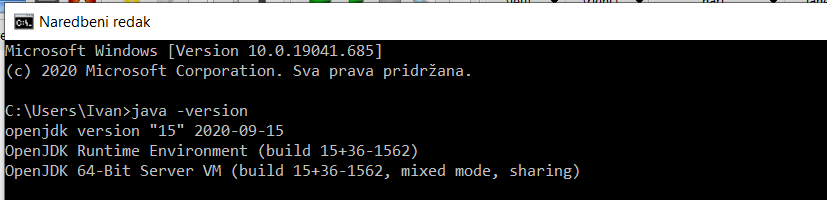
\includegraphics[scale=0.6]{slike/Java.PNG} %veličina slike u odnosu na originalnu datoteku i pozicija slike
				\centering
				\caption{Provjera instalacije Jave}
				\label{fig:java}
			\end{figure}
			
			Kako se uz Javu koristi i programski jezik JavaScript potrebno je instalirati i njegovu podršku odnosno potrebno je instalirati Node.js. Poveznica za instalaciju Node.js-a: \url{https://nodejs.org/en/download/} te je dana u popisu literature te se jednostavno uz pomoć uputa instalira. Također je potrebno provjeriti uspješnost instaliranja Node.js-a u naredbenom retku naredbom: " node -v".
			
			\begin{figure}[H]
				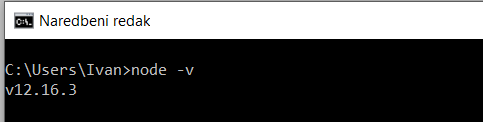
\includegraphics[scale=0.6]{slike/node.PNG} %veličina slike u odnosu na originalnu datoteku i pozicija slike
				\centering
				\caption{Provjera instalacije Node.js-a}
				\label{fig:node}
			\end{figure}
		
		Kada je sve to spremno potrebno je instalirati razvojnu okolinu koja nam pomaže pri izradi same aplikacije i njenog pokretanja. Primjer jedne takve okoline je Intelij IDE koji je za studente FER-a besplatan, no moguće je koristiti i druge razvojne okoline poput Eclipsa. Poveznica za preuzimanje ove razvojne okoline:  \url{https://www.jetbrains.com/idea/download/#section=windows}  također se nalazi i u popisu literature.
		
		Uz to za preuzimanje projekta možete se poslužiti sa Git GUI-em kojega je moguće preuzeti sa slijedeće poveznice: \url{https://git-scm.com/downloads}. Međutim možete samo skinuti projekt sa \url{https://gitlab.com/ivicamarica/ivicamarica} te ga pohraniti na željeno mjesto.
		
		Za kraj morate na svome računalu imati i program za upravljanje projektima, u ovom slučaju je to Gradle. \url{https://gradle.org/install/} je poveznica za prezimanje.
		
		Kada ste sve to pripremili konačno možete pokrenuti aplikaciju. Za uspješno pokretanje aplikacije potrebno je prvo instalirati npm pakete koji se koriste. To se treba učiniti pokretanjem naredbe
		npm install unutar direktorija src/main/js.
		Spring Boot aplikaciju je moguće pokrenuti unutar IDE-a ili naredbom gradle bootRun iz naredbenog retka.
		Frontend se pokreće naredbom npm start unutar direktorija src/main/js nakon čega se aplikacija može pregledavati u pregledniku na adresi http://localhost:3000.
		Nakon što ste ovako pokrenuli aplikaciju možete ju koristiti jer će se ona sama pobrinuti za sve potrebne komponente poput stvaranja baze i ostaloga.
		
		Ukoliko samo želite pogledati i isprobati aplikaciju, aplikacija je dostupna na poveznici  \url{https://progi-stop-waste.herokuapp.com/}.
		
		
		
		
			 
			
			\eject 